% ----------------------------- Design ---------------------------------------

\section{Design}

\subsection{Technical Environment}
% Mention minimum hardware configuration, software tools and package details.
\noindent
The technical environment for the project "Multimodal AI Framework for Social Media Based Mental Disorder Detection and Personalized Wellbeing Insights" comprises a combination of hardware, software, and tools that enable smooth data analysis, machine learning model training, and deployment. Below is an overview of the minimum hardware configuration, software tools, and package details necessary to carry out this project effectively. 

\begin{table}[h]
    \centering
    \renewcommand{\arraystretch}{1.2}
    \begin{tabular}{|c|p{12cm}|}
        \hline
        \textbf{Component} & \textbf{Specification} \\
        \hline
        Processor & Intel Core i5 (or equivalent) with a base clock speed of at least 2.5 GHz. A multi-core processor is preferred for parallel processing, essential for model training and data preprocessing. \\
        \hline
        RAM & 8 GB recommended for handling data loading, cleaning, and transformation. For large datasets, 16 GB is ideal to prevent memory overflow and processing delays. \\
        \hline
        Storage & Minimum 256 GB SSD recommended. SSD offers faster read/write speeds, significantly improving dataset loading times, especially for large datasets like Reddit-based social media posts. \\
        \hline
        GPU & Not necessary for basic ML tasks like Logistic Regression or SVM. For deep learning, an NVIDIA GTX 1060 with 4 GB VRAM or higher is advantageous. \\
        \hline
        Operating System & Windows 10 (64-bit) or higher, macOS 10.13 (High Sierra) or higher, or any stable Linux distribution (e.g., Ubuntu 18.04 or higher). The OS should support ML libraries and project tools. \\
        \hline
    \end{tabular}
    \caption*{\textbf{Minimum Hardware Configuration}}
\end{table}


\begin{table}[h]
    \centering
    \renewcommand{\arraystretch}{1.2}
    \begin{tabular}{|c|p{12cm}|}
        \hline
        \textbf{Library/Package} & \textbf{Description} \\
        \hline
        Python & Primary programming language for data processing and model training. \\
        \hline
        pandas & Data manipulation and preprocessing. \\
        \hline
        scikit-learn & Machine learning models and evaluation tools. \\
        \hline
        Streamlit & Web framework for deploying interactive ML applications. \\
        \hline
        pyngrok & Creates secure tunnels for sharing local applications. \\
        \hline
        Google Colab & Cloud-based Python environment with GPU/TPU support. \\
        \hline
        PRAW & Access and retrieve Reddit data via API. \\
        \hline
        pytesseract & OCR library for extracting text from images. \\
        \hline
        Pillow & Image processing and handling library. \\
        \hline
    \end{tabular}
    \caption*{\textbf{Libraries and Packages Used}}
    \label{tab:libraries}
\end{table}

\pagebreak
\begin{table}[H]
    \centering
    \renewcommand{\arraystretch}{1.2}
    \begin{tabular}{|c|p{12cm}|}
        \hline
        \textbf{Library/Package} & \textbf{Description} \\
        \hline
        joblib & Serialization and model saving utility. \\
        \hline
        protobuf & Efficient data serialization format by Google. \\
        \hline
        deep-translator & Multilingual text translation. \\
        \hline
        Requests & Library for making HTTP requests. \\
        \hline
        google-generativeai & Integrate Google’s generative AI models. \\
        \hline
        ffmpeg & Multimedia framework for processing audio/video. \\
        \hline
        tesseract-ocr & OCR tool for text extraction. \\
        \hline
        portaudio19-dev & Required for handling audio input/output. \\
        \hline
        poppler-utils & Converts PDFs to images for text extraction. \\
        \hline
        pydub & Audio processing library. \\
        \hline
        sounddevice & Real-time audio recording/playback. \\
        \hline
        wavio & WAV file handling. \\
        \hline
        numpy & Numerical computing library. \\
        \hline
        PyAudio & Audio input/output handling. \\
        \hline
        SpeechRecognition & Converts speech to text. \\
        \hline
        pdf2image & Converts PDFs to images. \\
        \hline
        tweepy & Access and analyze Twitter data. \\
        \hline
        openai-whisper & Speech-to-text model from OpenAI. \\
        \hline
        tiktoken & Tokenizer for language models. \\
        \hline
        librosa & Audio analysis and feature extraction. \\
        \hline
        opencv-python & Computer vision and image processing. \\
        \hline
        xgboost & Gradient boosting for ML models. \\
        \hline
        deepface & Facial recognition and emotion analysis. \\
        \hline
        tf\_keras & Keras API for TensorFlow. \\
        \hline
        transformers & Pre-trained NLP models from Hugging Face. \\
        \hline
        tensorflow & Deep learning framework. \\
        \hline
        nltk & Natural language processing toolkit. \\
        \hline
        plotly & Interactive data visualization. \\
        \hline 
        matplotlib & Static and animated plots. \\
        \hline
        scipy & Scientific computing and signal processing. \\
        \hline
        networkx & Graph analysis and visualization. \\
        \hline
        yt-dlp & YouTube video/audio downloader. \\
        \hline
    \end{tabular}
    \caption*{\textbf{Libraries and Packages Used}}
    \label{tab:libraries}
\end{table}

\pagebreak

\subsection{Hierarchy of Modules}
% Provide a diagram.
\begin{figure}[h!]  
    \centering
    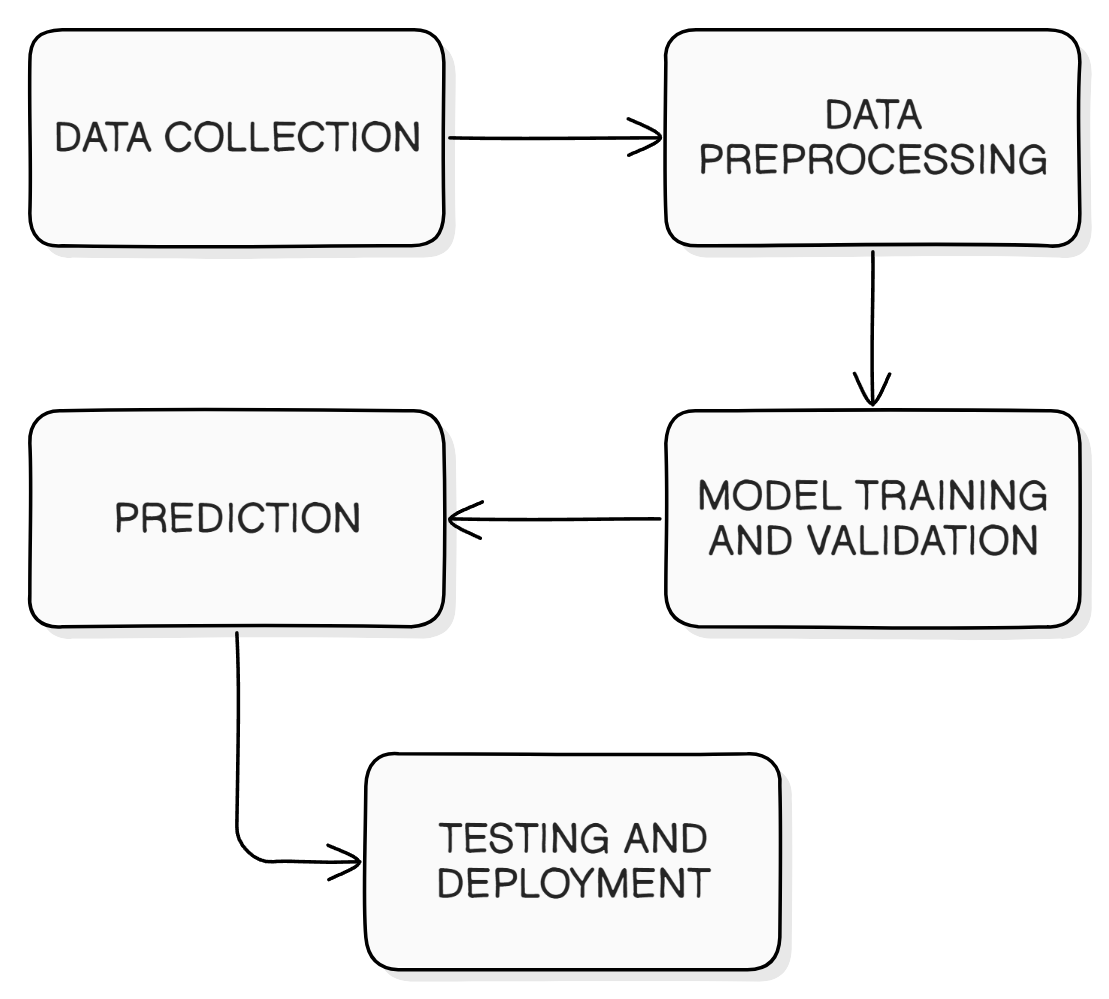
\includegraphics[width=0.5\textwidth]{Images/Project Modules.png}  
    \caption*{Project Modules}
    \label{Project Modules}  % Label for referencing the figure
\end{figure}

\begin{table}[H]
    \centering
    \renewcommand{\arraystretch}{1.2} % Adjust row height for better readability
    \small % Reduce text size to fit within the page
    \begin{tabularx}{\textwidth}{|p{3.5cm}|X|}
        \hline
        \textbf{Module} & \textbf{Description} \\
        \hline
        \textbf{Data Collection} & Gathers relevant text data from posts in platforms like Reddit via PRAW. \\
        \hline
        \textbf{Data Preprocessing} & Cleans and prepares text data using:
        \begin{itemize}
            \setlength{\itemsep}{0pt}  % Adjust spacing between items
            \setlength{\parskip}{0pt}
            \item Tokenization (splitting text into words/tokens)
            \item Lowercasing for uniformity
            \item Stop-word removal
            \item Lemmatization or stemming
        \end{itemize} \\
        % \hline
        \textbf{} & Perform feature extraction to convert text into numerical features using:
        \begin{itemize}
            \setlength{\itemsep}{0pt}  % Adjust spacing between items
            \setlength{\parskip}{0pt}
            \item Term Frequency-Inverse Document Frequency (TF-IDF)
            \item Bag of Words (BoW) model
            \item Word2Vec, LIWC (Linguistic Inquiry and Word Count) and N-Gram were also explored
        \end{itemize} \\
        \hline
        \textbf{Model Training and Validation} & Splits dataset into training/testing sets and trains models such as:
        \setlength{\itemsep}{0pt}  % Adjust spacing between items
        \setlength{\parskip}{0pt}
        \begin{itemize}
            \item Logistic Regression, Naive Bayes, SVM, XGBoost, KNN, LSTM, Transformer. These formed the base models for the ensemble model used in application where Random Forest was used as the meta-learner All were validated to assess performance.
        \end{itemize} \\
        \hline
        \textbf{Prediction} & Processes received and combined text input for classification using trained models. \\
        \hline
        \textbf{Testing and Deployment} & Deploys models on Streamlit Cloud for real-time predictions and wellbeing insights using association matrix. Provides a user interface for easy access. \\
        \hline
    \end{tabularx}
    \caption*{\textbf{Hierarchy of Modules in the system}}
    \label{tab:modules_hierarchy}
\end{table}


\subsection{Detailed Design}
% Provide hierarchy of modules or overall system diagram. 
% \vspace{.1in}
\begin{figure}[h!]  
    \centering
    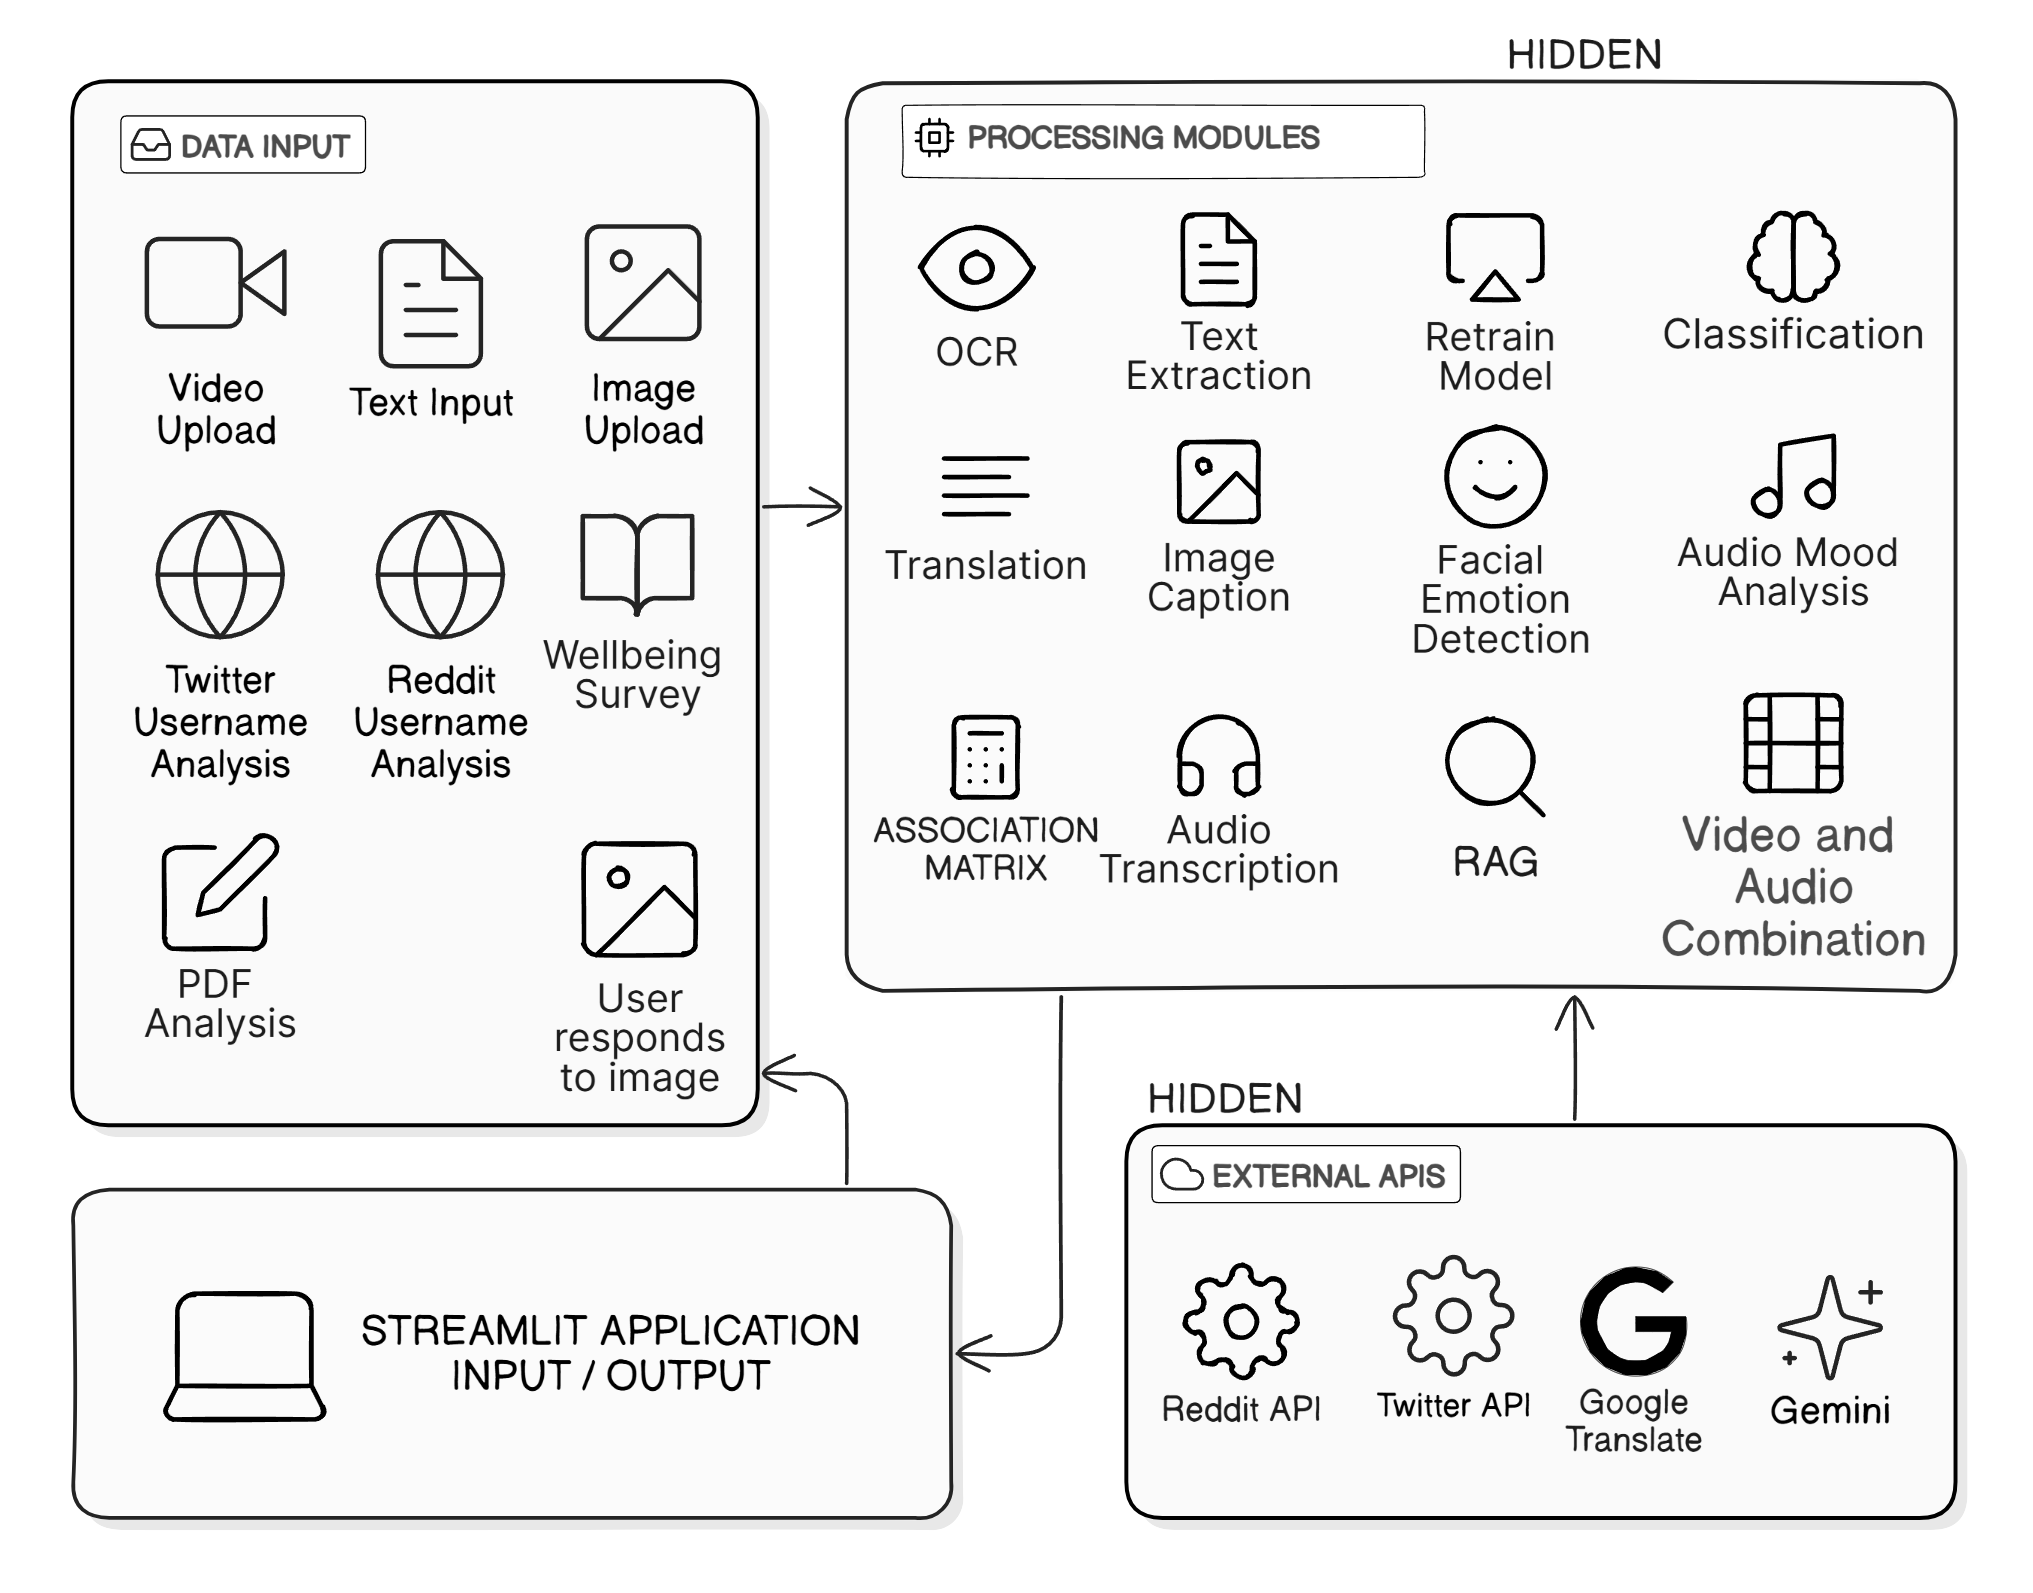
\includegraphics[width=0.85\textwidth]{Images/System Overview.png}  
    \caption*{System Overview}
    \label{System Overview}  % Label for referencing the figure
\end{figure}

\begin{figure}[h!]  
    \centering
    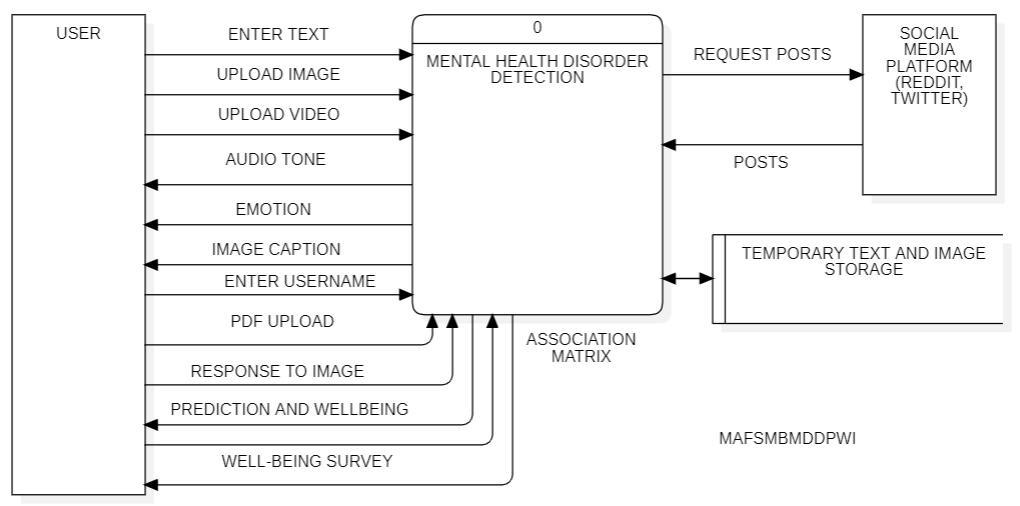
\includegraphics[width=0.85\textwidth]{Images/DFD L0.png}  
    \caption*{DFD Level 0 of the System}
    \label{dfdl0123}  % Label for referencing the figure
\end{figure}

\pagebreak

\begin{figure}[h!]  
    \centering
    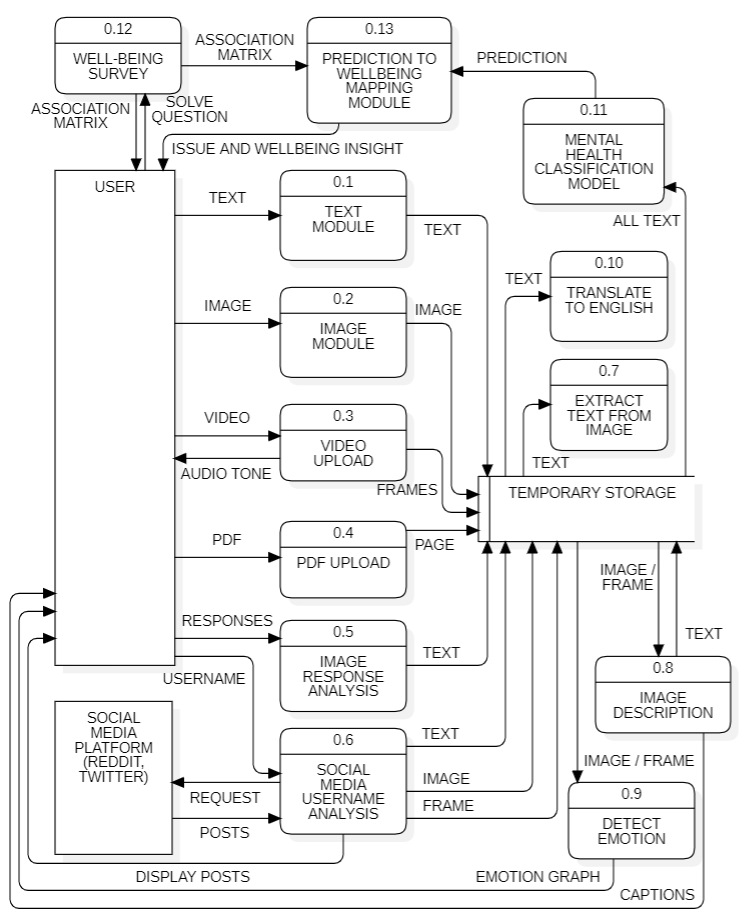
\includegraphics[width=0.725\textwidth]{Images/DFD L1.png}  
    \caption*{DFD Level 1 of the System}
    \label{dfdl1234}  % Label for referencing the figure
\end{figure}

\vspace{2em}

\noindent
\textbf{Image Description}

\begin{figure}[h!]  
    \centering
    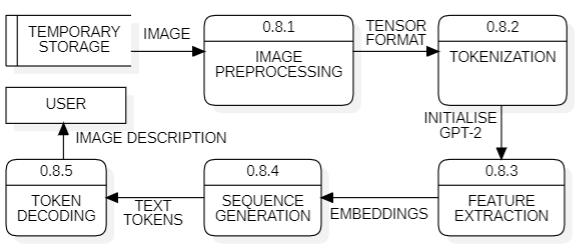
\includegraphics[width=0.7\textwidth]{Images/DFD L2 ID.png}  
    \caption*{DFD Level 2 of Image Description}
    \label{dfdl122}  % Label for referencing the figure
\end{figure}

\noindent
The image captioning process using Python’s Transformers module and the ViT-GPT2 model involves several key steps. The user uploads an image, which is preprocessed by resizing to \(224 \times 224\) pixels, normalizing pixel values, and converting it into a tensor format. The Vision Transformer (ViT) divides the image into \(16 \times 16\) patches, embeds them, and processes them through transformer layers to extract visual features. The resulting embedding is passed to GPT-2, which generates a sequence of text tokens iteratively using its language model. Tokens are decoded back into human-readable text using the GPT-2 tokenizer, cleaned for readability, and output as a concise description. This pipeline leverages ViT for feature extraction and GPT-2 for language generation, enabling efficient and almost accurate image captioning.

\vspace{2em}

\noindent
\textbf{Emotion Detection Functionality}

\begin{figure}[h!]  
    \centering
    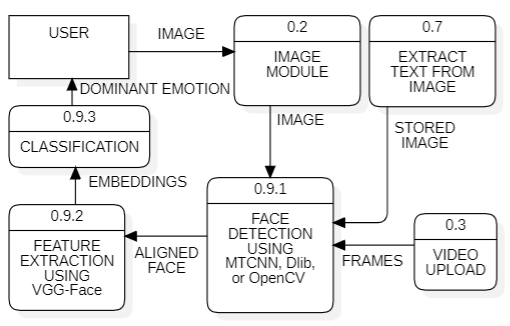
\includegraphics[width=0.7\textwidth]{Images/DFD L2 EMOTION.png}  
    \caption*{DFD Level 2 of Emotion Detection Functionality}
    \label{dfdl14456}  % Label for referencing the figure
\end{figure}

\noindent
DeepFace analysis processes facial features from uploaded images or video frames through a structured pipeline. It starts with face detection using models like MTCNN, Dlib, or OpenCV to locate and align faces. The detected faces are cropped and passed to feature extraction, where pre-trained models like VGG-Face or Facenet generate numerical embeddings. These embeddings are compared using cosine similarity or Euclidean distance for tasks like emotion detection (e.g., happiness, sadness), demographic analysis (e.g., age, gender), or face verification. The results, such as detected emotions or attributes, are then displayed to the user. This process enables real-time analysis of facial expressions and emotions, providing valuable insights for mental health monitoring and wellbeing assessment.

\pagebreak

\noindent
\textbf{Extract Text From Image}

\begin{figure}[h!]  
    \centering
    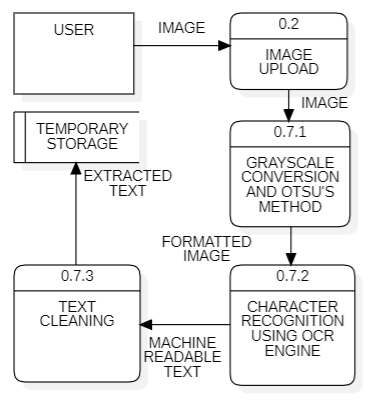
\includegraphics[width=0.5\textwidth]{Images/DFD L2 TEXT EXTRACT.png}  
    \caption*{DFD Level 2 of Text Extraction from Image}
    \label{dfdl13456}  % Label for referencing the figure
\end{figure}

\noindent
The process of extracting text from an image using Tesseract-OCR begins with preprocessing the uploaded image. The image is converted to grayscale, noise is reduced using Gaussian or Median Blur, and binarization (e.g., Otsu’s thresholding) isolates text from the background. Text regions are detected using contour analysis or connected components. The processed image is then passed to Tesseract, which uses an LSTM-based neural network to recognize characters and generate machine-readable text, enhanced by language models for accuracy. Postprocessing corrects errors via spell-checking and rule-based replacements (e.g., \texttt{0} $\rightarrow$ \texttt{O}), and formats the text into paragraphs or lines. The final output, displayed or saved as \texttt{.txt} or \texttt{.docx}, is ready for applications like document analysis. This pipeline combines image enhancement, deep learning, and text correction for high-quality results.

\vspace{2em}

\noindent
\textbf{Translation to English}

\begin{figure}[h!]  
    \centering
    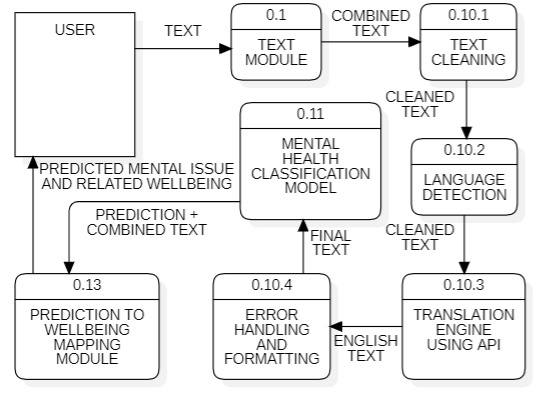
\includegraphics[width=0.7\textwidth]{Images/DFD L2 TE.png}  
    \caption*{DFD Level 2 of Translation to English}
    \label{dfdl111}  % Label for referencing the figure
\end{figure}

\noindent
The process of translating text to English using DeepTranslator begins with preprocessing the input to clean unwanted characters and detect the source language using machine learning models like Google’s Compact Language Detector. The prepared text is passed to DeepTranslator, which interfaces with APIs like Google Translate or Microsoft Translator. These APIs use neural machine translation (NMT) with encoder-decoder architectures and attention mechanisms to translate the text into English. Transformer-based models enhance accuracy by capturing context and long-range dependencies. Postprocessing ensures quality by validating completeness, correcting errors, and preserving formatting. The final translated text is displayed or saved, ensuring accuracy and readability. This pipeline integrates NLP, deep learning, and error handling for reliable translations.

\vspace{2em}

\noindent
\textbf{Audio Mood Analysis}

\begin{figure}[h!]  
    \centering
    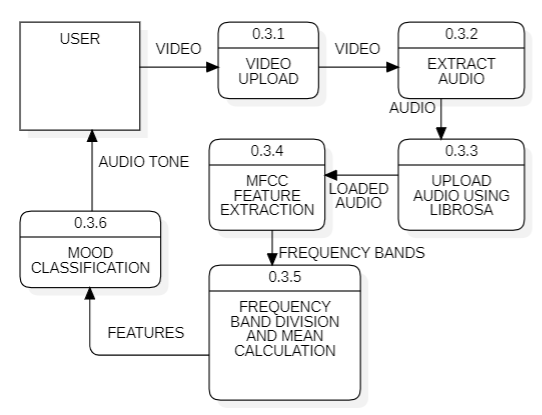
\includegraphics[width=0.7\textwidth]{Images/DFD L2 AM.png}  
    \caption*{DFD Level 2 of Audio Mood Analysis}
    \label{dfdl671}  % Label for referencing the figure
\end{figure}

\pagebreak

\noindent
The \texttt{analyze\_audio\_mood} function begins with the user providing a video file path. The audio is extracted using the \texttt{extract\_audio\_from\_video} function and loaded into memory with the Librosa library. Mel-frequency cepstral coefficients (MFCCs) are computed using \texttt{librosa.feature.mfcc} to capture frequency patterns for mood analysis. The MFCC array is segmented into four frequency bands—low, mid-low, mid-high, and high—and the scalar mean of each band is calculated to simplify data for classification. The mood is classified (e.g., normal, calm, anxious) based on the dominant frequency characteristics. Results can be further enhanced using the Gemini API to provide tone, mood, and summary details for the audio. This process combines audio feature extraction and classification for comprehensive mood analysis.

\vspace{2em}

\noindent
\textbf{Prediction to Wellbeing Mapping}

\begin{figure}[h!]  
    \centering
    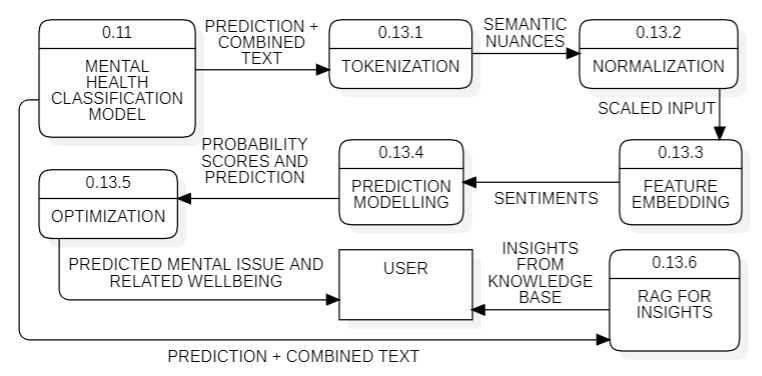
\includegraphics[width=0.7\textwidth]{Images/DFD L2 MW.png}  
    \caption*{DFD Level 2 of Prediction to Wellbeing Mapping}
    \label{dfdl166}  % Label for referencing the figure
\end{figure}

\noindent
The system first processes user input (text, behavioral data, or health metrics) through preprocessing and feature extraction. Machine learning models then predict the most likely mental health condition along with associated probabilities. The top predicted issue and its probability are then fed into GEMINI 2.0 FLASH with a structured prompt to generate wellbeing insights based on Ryff’s six parameters. To refine these insights, an association matrix maps the probabilities of all predicted issues to specific wellbeing parameters, selecting 1 to 3 key parameters (e.g., autonomy, personal growth, or self-acceptance). This ensures that the user receives targeted recommendations for improving their psychological wellbeing. There is also an additional feature where Retrieval Augmented Generation (RAG) is used to provide personalized recommendations based on the user’s mental health condition. The system retrieves relevant information from a knowledge base and generates tailored suggestions.
\vspace{1em}

\noindent
The above 6 main functionalities are reused in the application for the options available to the user. These include \textbf{Text} analysis, \textbf{Image} analysis, \textbf{Video} analysis, \textbf{PDF} analysis, analysis of \textbf{User response to Image}, analysis of \textbf{Reddit} and \textbf{Twitter} user profiles. \textbf{Wellbeing Survey Option} and \textbf{RAG for wellbeing Insights} have been added under \textit{Implementation} section.

\vspace{1em}

\noindent
Below are the flow diagrams for the various \textit{Analysis} options that the web application provides.

\begin{figure}[H]  
    \centering
    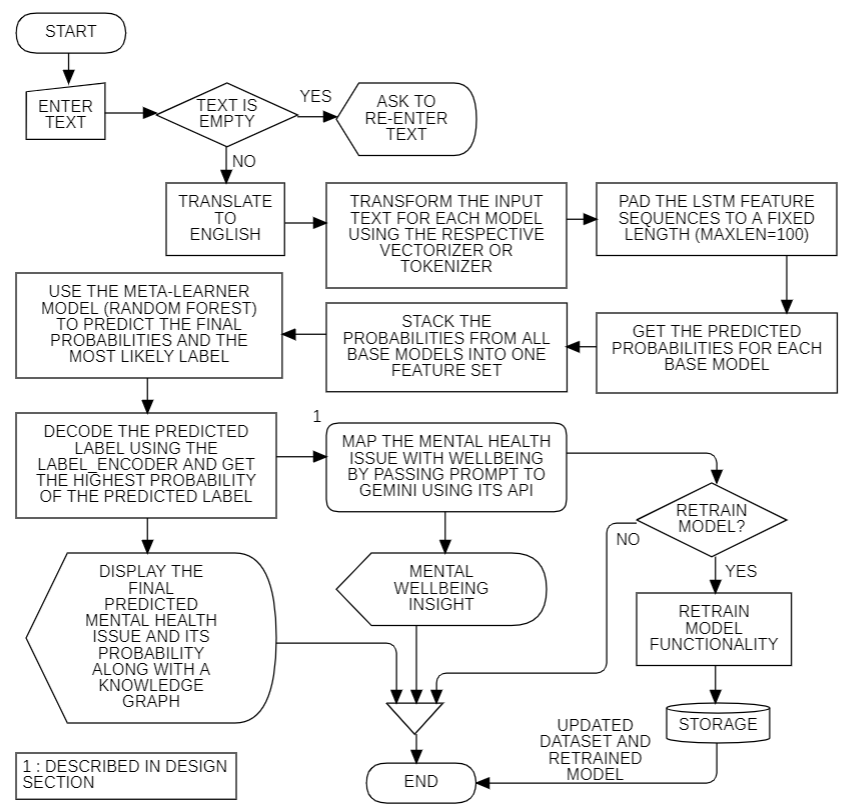
\includegraphics[width=0.72\textwidth]{Images/APP TEXT OPTION.png}  
    \caption*{Text Classification Flow Diagram}
    \label{012i}  % Label for referencing the figure
\end{figure}

% -- pdf upload
\begin{figure}[H]  
    \centering
    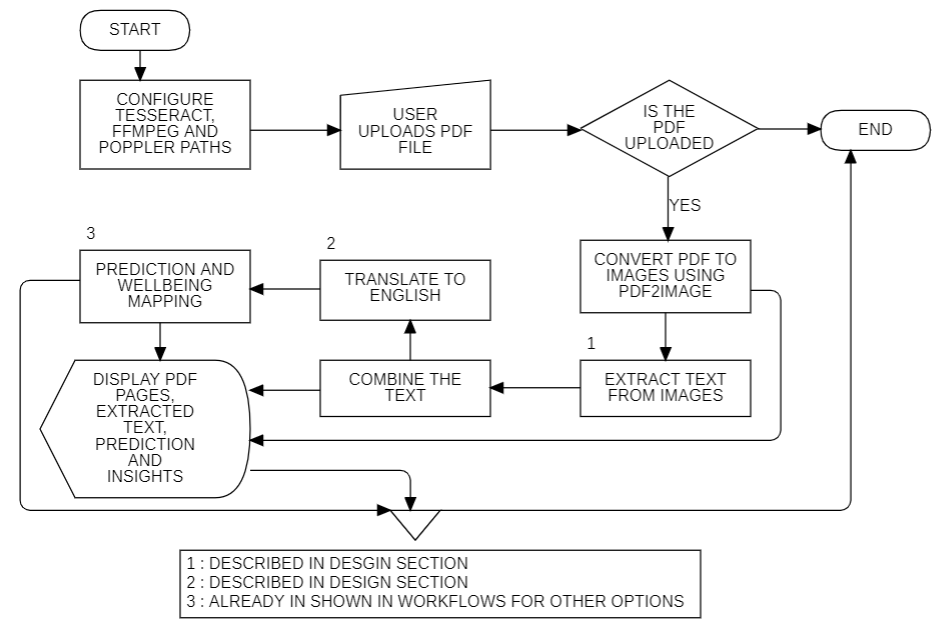
\includegraphics[width=0.72\textwidth]{Images/APP PDF.png}  
    \caption*{PDF Upload Flow Diagram}
    \label{01234i}  % Label for referencing the figure
\end{figure}

\pagebreak

\begin{figure}[H]  
    \centering
    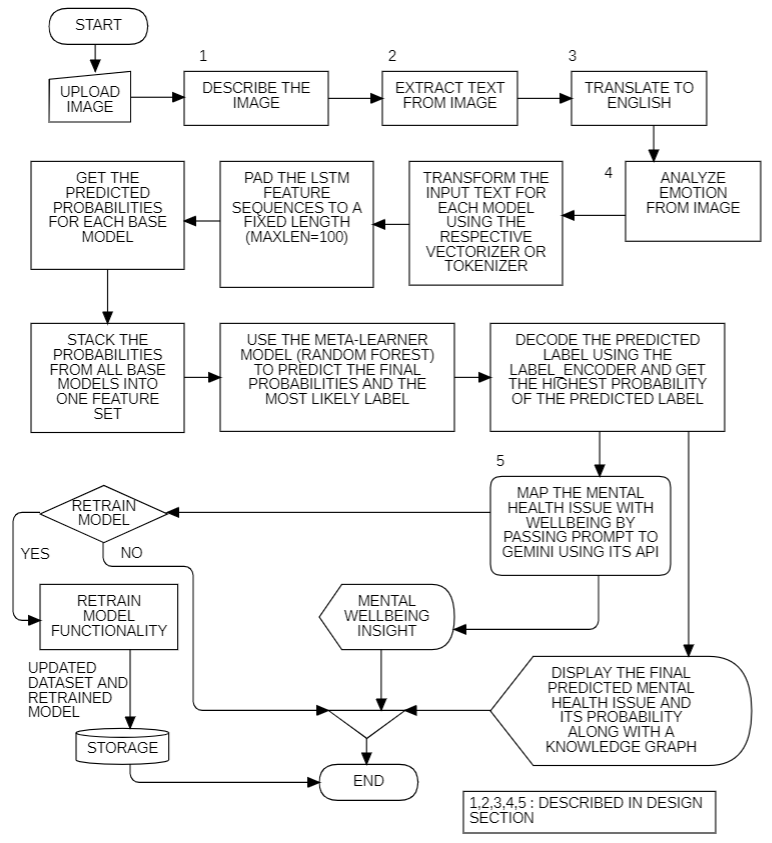
\includegraphics[width=0.77\textwidth]{Images/APP IMAGE OPTION.png}  
    \caption*{Image Classification Flow Diagram}
    \label{011232i}  % Label for referencing the figure
\end{figure}

% -- user response to image
\begin{figure}[H]  
    \centering
    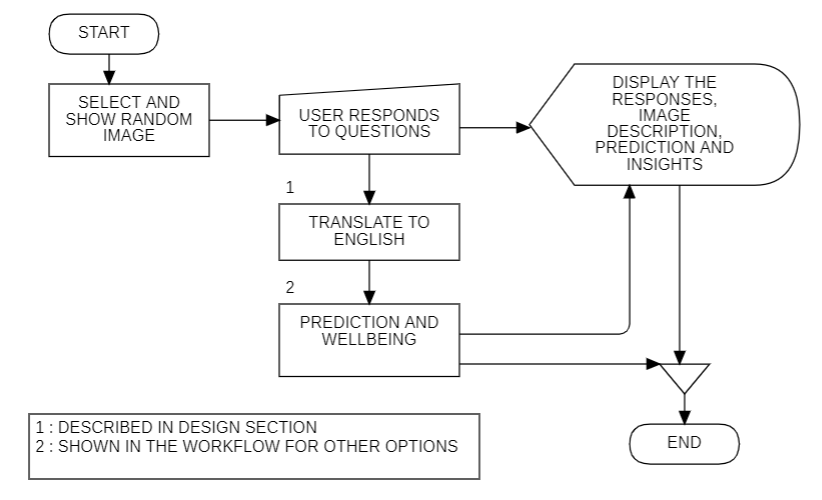
\includegraphics[width=0.77\textwidth]{Images/APP RESPOND.png}  
    \caption*{User Response to Image Flow Diagram}
    \label{01234i}  % Label for referencing the figure
\end{figure}

\pagebreak



\vfill
\begin{figure}[H]
    \centering
    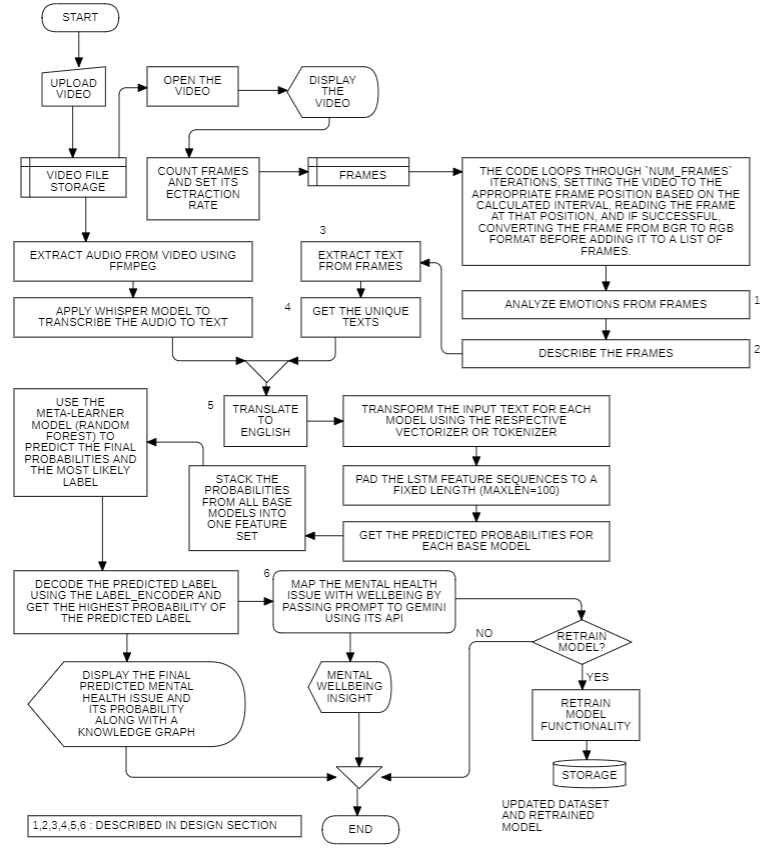
\includegraphics[width=1.0\textwidth]{Images/APP VIDEO OPTION.png}
    \caption*{Video Classification Flow Diagram}
    \label{01332i}
\end{figure}
\vfill


\pagebreak
\begin{figure}[h!]  
    \centering
    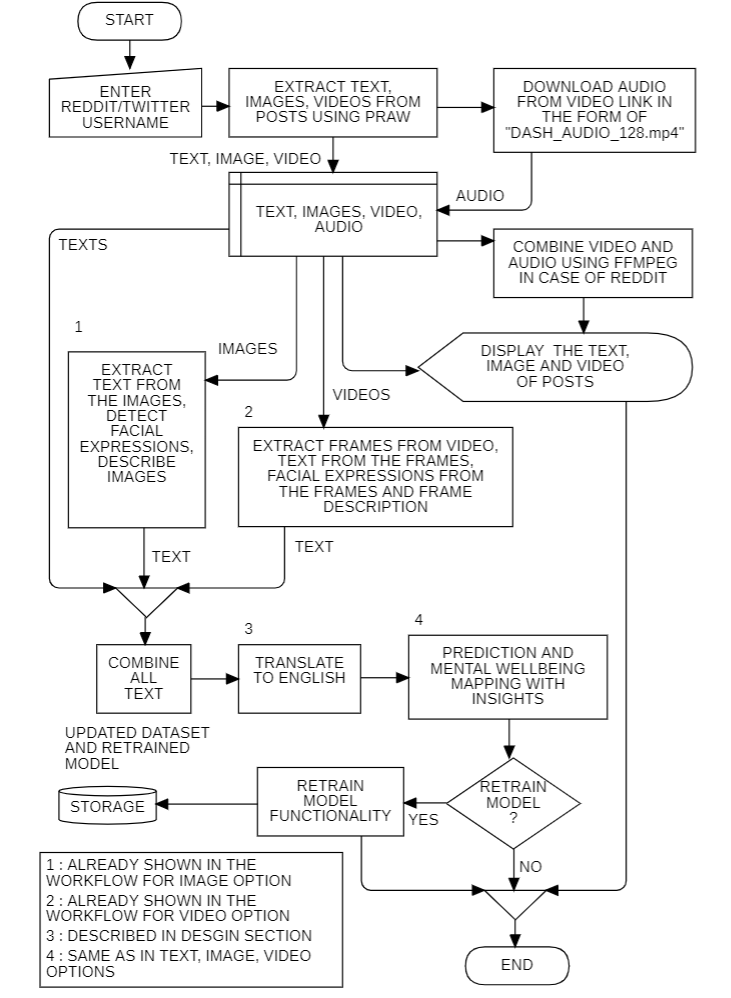
\includegraphics[width=0.9\textwidth]{Images/APP REDDIT.png}  
    \caption*{Reddit and Twitter username Classification Flow Diagram}
    \label{01234i}  % Label for referencing the figure
\end{figure}


\pagebreak


% \noindent
% Create separate sections for separate modules of design as in Requirement Matrix. Ensure to provide Design Diagrams \textit{(e.g. System overview / DFDs / ERDs etc.; cross-reference to be drawn from Chapter 6), Decision matrix (for algorithm recommendation etc.) }




% \subsubsection{Name of Design Module 1 \label{sec:design_mod1}}
% \subsubsection{Name of Design Module 2 \label{sec:design_mod2}}
% \subsubsection{Name of Design Module 3 etc \label{sec:design_mod3}}


% Refer APPENDIX A  – Prototypes \ref{sec:proto} for prototype details.


% ------------------------------ Design Ends ---------------------------------

